\chapter{Plantas sin semillas}\label{ch:g4:plants-without-seeds}

La cara sombría del muro viejo está tapizada de musgo; bajo las hayas,
los \omterm{prop:g4:plants-without-seeds:damp}{helechos} despliegan sus grandes frondas verdes. Búscales todo el
verano: no encontrarás ni una \omterm{def:g3:flowers-fruits-seeds:parts}{flor}, ni un \omterm{prop:g3:flowers-fruits-seeds:transform}{fruto}, ni una \omterm{def:g2:from-seed-to-plant:seed}{semilla} ---
nunca. Y sin embargo el musgo y los \omterm{prop:g4:plants-without-seeds:damp}{helechos} se extienden
estupendamente. Resulta que las \omterm{def:g1:plants-around-us:plant}{plantas} tienen más de una manera de
hacer la generación siguiente.

\section{Helechos y musgos: reproducción por esporas}

\begin{definition}[Espora]\label{def:g4:plants-without-seeds:spore}
Una \emph{espora}\index{espora} es un granito microscópico, fabricado
en cantidades enormes, del que puede salir una \omterm{def:g1:plants-around-us:plant}{planta} nueva. A
diferencia de una \omterm{def:g2:from-seed-to-plant:seed}{semilla} (\cref{def:g2:from-seed-to-plant:seed}), una
espora es una mota suelta \emph{sin despensa y sin ninguna plantita ya
hecha dentro} --- es un comienzo en lo más escueto.
\end{definition}

\begin{example}[Bajo las frondas del helecho]\label{ex:g4:plants-without-seeds:fern}
Dale la vuelta a una fronda de helecho a finales de verano: filas
ordenadas de puntos marrones recorren su envés. Cada punto es un
paquete de miles de \omterm{def:g4:plants-without-seeds:spore}{esporas}; cuando maduran, los paquetes se abren y
las \omterm{def:g4:plants-without-seeds:spore}{esporas} se van con el aire como el polvo más fino. Una \omterm{def:g4:plants-without-seeds:spore}{espora} que
cae en un suelo húmedo y sombrío puede convertirse --- por etapas ---
en un helecho nuevo.
\end{example}

\begin{omfigure}
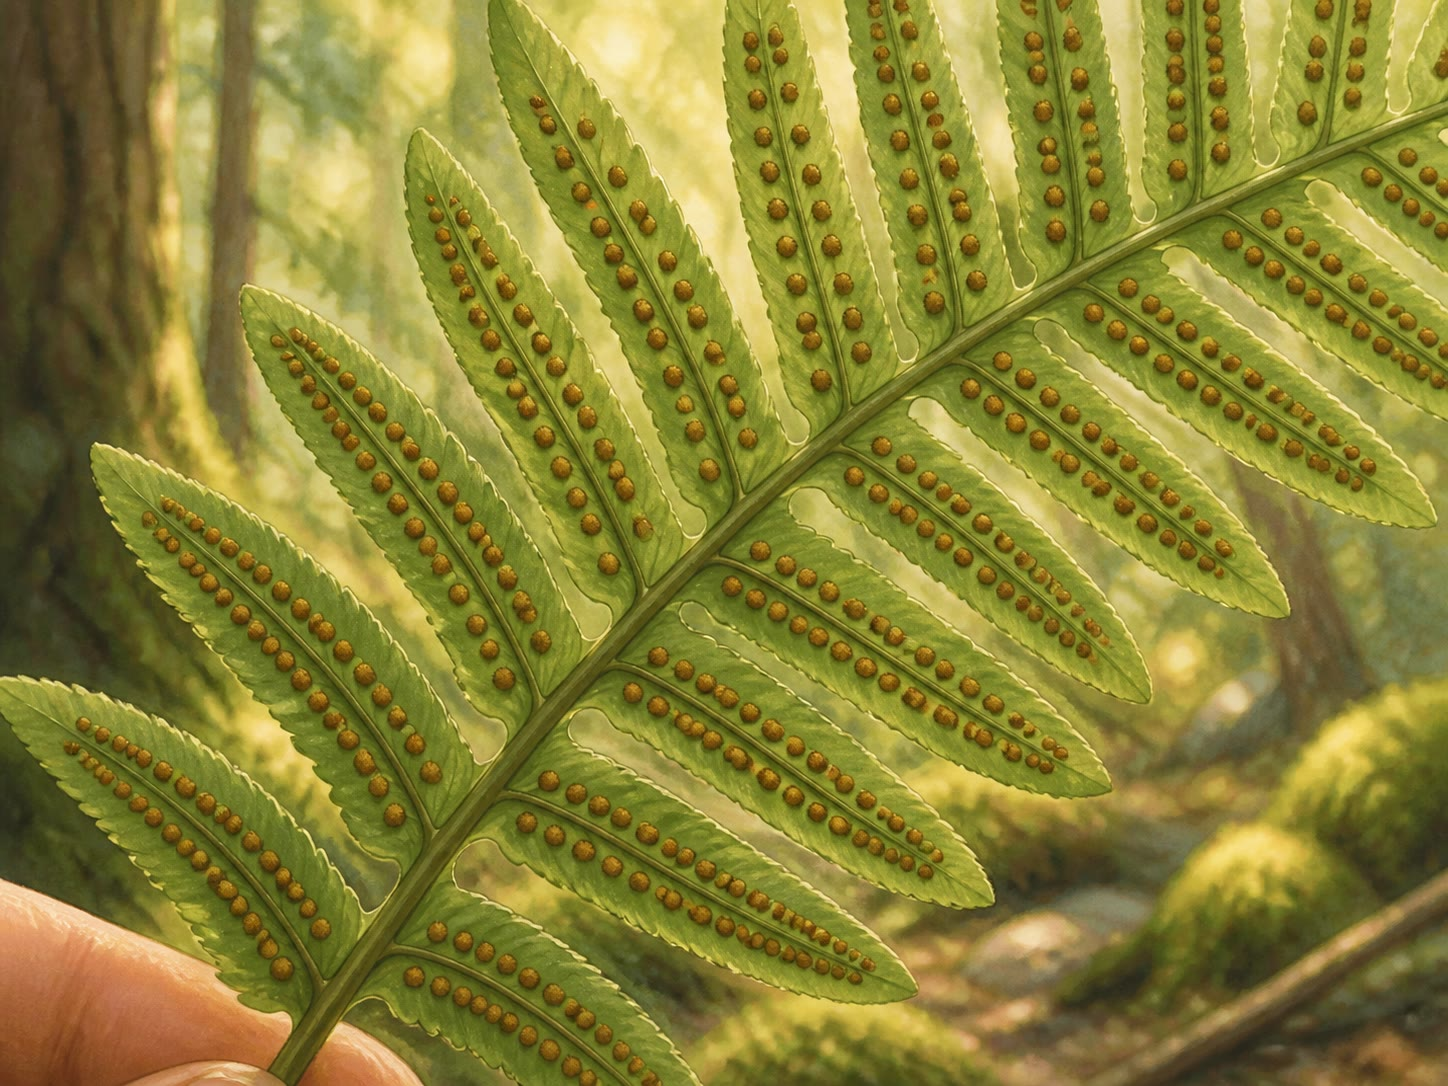
\includegraphics[width=0.56\linewidth]{images/book1/ai/g4-ferns-sori.jpg}

{\small Bajo la fronda: las filas ordenadas de puntos marrones, cada
uno un paquete de miles de \omterm{def:g4:plants-without-seeds:spore}{esporas}.}
\end{omfigure}

\begin{proposition}[Las plantas de esporas necesitan humedad]\label{prop:g4:plants-without-seeds:damp}
Las \omterm{def:g1:plants-around-us:plant}{plantas} de \omterm{def:g4:plants-without-seeds:spore}{esporas} --- \emph{musgos}\index{musgo} y
\emph{helechos}\index{helecho} --- solo se pueden reproducir donde hay
\emph{humedad}: sus \omterm{def:g4:plants-without-seeds:spore}{esporas}, y las etapas delicadas que salen de
ellas, se secan y se mueren en el aire seco. Por eso el musgo
tapiza el muro norte sombrío y nunca el muro sur soleado, y por eso
los \omterm{prop:g4:plants-without-seeds:damp}{helechos} se apiñan en bosques húmedos, orillas de arroyo y pozos.
\end{proposition}
\admitted

\begin{remark}[Una espora no es una semilla]\label{rem:g4:plants-without-seeds:sporeseed}
Las dos son comienzos que viajan, pero la \omterm{def:g2:from-seed-to-plant:seed}{semilla} es un equipo de
supervivencia --- cubierta, despensa, plantita ya hecha --- mientras
que la \omterm{def:g4:plants-without-seeds:spore}{espora} va desnuda. De ahí las cifras: los millones de \omterm{def:g4:plants-without-seeds:spore}{esporas}
del helecho frente a la docena de \omterm{prop:g3:flowers-fruits-seeds:transform}{semillas} de la vaina de judías. Los
comienzos desnudos son baratos de hacer y fáciles de perder; los dos
planes son el eco del bacalao y de la elefanta de la
\cref{prop:g4:animal-reproduction:strategies}.
\end{remark}

\section{Plantas nuevas sin sembrar nada}

\begin{definition}[Reproducción vegetativa]\label{def:g4:plants-without-seeds:vegetative}
Muchas \omterm{def:g1:plants-around-us:plant}{plantas} pueden además hacer \omterm{def:g1:plants-around-us:plant}{plantas} nuevas \emph{directamente a
partir de un trozo de sí mismas} --- sin \omterm{def:g4:plants-without-seeds:spore}{esporas}, sin \omterm{prop:g3:flowers-fruits-seeds:transform}{semillas} y con
un solo progenitor. Eso es la \emph{reproducción
vegetativa}\index{reproducción vegetativa}. La \omterm{def:g1:plants-around-us:plant}{planta} nueva es una
continuación viva de la vieja, y se le parece exactamente.
\end{definition}

\begin{example}[Los estolones de la fresa]\label{ex:g4:plants-without-seeds:runner}
Una mata de fresas echa \omterm{def:g1:plants-around-us:parts}{tallos} horizontales largos y finos --- los
\emph{estolones}\index{estolón} --- por encima de la tierra. Donde un
estolón toca el suelo, echa \omterm{def:g1:plants-around-us:parts}{raíces}, saca \omterm{def:g1:plants-around-us:parts}{hojas} y se convierte en una
mata de fresas nueva y completa; después el estolón se marchita y la
hija queda libre. Una \omterm{def:g1:plants-around-us:plant}{planta} se convierte en un fresal sin sembrar ni
una \omterm{def:g2:from-seed-to-plant:seed}{semilla}.
\end{example}

\begin{example}[Bulbos y tubérculos]\label{ex:g4:plants-without-seeds:bulbtuber}
El \emph{bulbo}\index{bulbo} del tulipán y el
\emph{tubérculo}\index{tubérculo} de la patata son almacenes
subterráneos --- y equipos de arranque. Si se dejan en la tierra, un
\omterm{ex:g4:plants-without-seeds:bulbtuber}{bulbo} se parte en \omterm{ex:g4:plants-without-seeds:bulbtuber}{bulbos} hijos, cada uno un tulipán futuro; y cada
``\omterm{def:g1:the-five-senses:sense}{ojo}'' de una patata brotada puede dar una \omterm{def:g1:plants-around-us:plant}{planta} entera nueva. Los
hortelanos plantan patatas, no \omterm{prop:g3:flowers-fruits-seeds:transform}{semillas} de patata.
\end{example}

\begin{method}[Hacer un esqueje]\label{met:g4:plants-without-seeds:cutting}
Los hortelanos copian la \omterm{def:g4:plants-without-seeds:vegetative}{reproducción vegetativa} con
\emph{esquejes}\index{esqueje}:
\begin{enumerate}
  \item corta de la \omterm{def:g1:plants-around-us:plant}{planta} madre un brote joven y sano, de un palmo
        (la menta, el sauce y los geranios van muy bien);
  \item quítale las \omterm{def:g1:plants-around-us:parts}{hojas} de abajo y pon el brote en agua o en tierra
        húmeda;
  \item espera: en días o semanas salen \omterm{def:g1:plants-around-us:parts}{raíces} del \omterm{def:g1:plants-around-us:parts}{tallo} cortado;
  \item plántalo --- una \omterm{def:g1:plants-around-us:plant}{planta} nueva y completa, idéntica a su único
        progenitor.
\end{enumerate}
\end{method}

\begin{remark}[Un progenitor, copias exactas]\label{rem:g4:plants-without-seeds:copy}
Las \omterm{prop:g3:flowers-fruits-seeds:transform}{semillas} mezclan dos progenitores (la
\cref{rem:g4:animal-reproduction:mix} vale también para las \omterm{def:g1:plants-around-us:plant}{plantas}, a
través del \omterm{def:g3:flowers-fruits-seeds:parts}{polen}); la \omterm{def:g4:plants-without-seeds:vegetative}{reproducción vegetativa} copia a uno. Por eso
todas las \omterm{def:g1:plants-around-us:plant}{plantas} de una variedad de manzana con nombre se cultivan a
partir de \omterm{met:g4:plants-without-seeds:cutting}{esquejes} e injertos, nunca de pepitas: el huerto quiere
copias exactas de un árbol excelente. El precio de copiar es la
igualdad --- un huerto de árboles idénticos comparte debilidades
idénticas, como enseñará un curso posterior.
\end{remark}

\section{Ejercicios}

\begin{exercise}[$\star$]\label{exo:g4:plants-without-seeds:1}
Nombra dos \omterm{def:g1:plants-around-us:plant}{plantas} que no hagan nunca \omterm{prop:g3:flowers-fruits-seeds:transform}{semillas}. ¿Cómo se reproducen?
\end{exercise}

\begin{exercise}[$\star$]\label{exo:g4:plants-without-seeds:2}
Da dos diferencias entre una \omterm{def:g4:plants-without-seeds:spore}{espora} y una \omterm{def:g2:from-seed-to-plant:seed}{semilla}.
\end{exercise}

\begin{exercise}[$\star$]\label{exo:g4:plants-without-seeds:3}
¿Dónde se fabrican las \omterm{def:g4:plants-without-seeds:spore}{esporas} del helecho? Describe lo que encuentras
bajo una fronda a finales de verano.
\end{exercise}

\begin{exercise}[$\star$]\label{exo:g4:plants-without-seeds:4}
¿Por qué crece el musgo en el muro norte sombrío y no en el muro sur
soleado?
\end{exercise}

\begin{exercise}[$\star$]\label{exo:g4:plants-without-seeds:5}
¿Qué es la \omterm{def:g4:plants-without-seeds:vegetative}{reproducción vegetativa}? ¿Cuántos progenitores hace falta?
\end{exercise}

\begin{exercise}[$\star$]\label{exo:g4:plants-without-seeds:6}
Cuenta la historia de un estolón de fresa, del primer \omterm{def:g1:plants-around-us:parts}{tallo} a la mata
hija que se sostiene sola.
\end{exercise}

\begin{exercise}[$\star$]\label{exo:g4:plants-without-seeds:7}
¿Por qué plantan patatas los hortelanos en vez de sembrar \omterm{prop:g3:flowers-fruits-seeds:transform}{semillas} de
patata? ¿Qué puede hacer cada ``\omterm{def:g1:the-five-senses:sense}{ojo}''?
\end{exercise}

\begin{exercise}[$\star$]\label{exo:g4:plants-without-seeds:8}
Pruébalo: haz un esqueje de menta con el
\cref{met:g4:plants-without-seeds:cutting} y ponlo en un vaso de agua
en el alféizar. ¿Qué aparece y al cabo de cuánto tiempo, más o menos?
\end{exercise}

\begin{exercise}[$\star\star$]\label{exo:g4:plants-without-seeds:9}
El helecho hace millones de \omterm{def:g4:plants-without-seeds:spore}{esporas}; la vaina de judías, una docena de
\omterm{prop:g3:flowers-fruits-seeds:transform}{semillas}. Explica la diferencia de números con la
\cref{rem:g4:plants-without-seeds:sporeseed} --- y nombra la pareja de
\omterm{def:g1:animals-around-us:animal}{animales} cuyas estrategias son su eco.
\end{exercise}

\begin{exercise}[$\star\star$]\label{exo:g4:plants-without-seeds:10}
Una hortelana se encuentra las matas de fresa nuevas idénticas a la
madre, mientras que sus judías varían un poco respecto de sus padres.
Explica las dos observaciones con la
\cref{rem:g4:plants-without-seeds:copy}.
\end{exercise}

\begin{exercise}[$\star\star\star$]\label{exo:g4:plants-without-seeds:11}
Una \omterm{def:g1:plants-around-us:tree}{rama} de sauce arrancada por una crecida de invierno, arrastrada
río abajo y varada en un banco de barro, se convierte a menudo en un
sauce nuevo. ¿Qué clase de reproducción es esta --- y por qué hay
tantos sauces en las orillas de los ríos? ¿Qué hizo la crecida que el
hortelano del \cref{met:g4:plants-without-seeds:cutting} hace con unas
tijeras?
\end{exercise}
